\documentclass[12pt]{article}                         
\pagestyle{plain}

\usepackage{amsmath}     % Enhanced math environments (e.g., align).
\usepackage{amsfonts}    % Math fonts (e.g., \mathfrak{}).
\usepackage{amstext}     % Text inside math mode (e.g., \text{where}).
\usepackage{amssymb}     % Extra math symbols (e.g., \mathbb{R}).
\usepackage{array}       % Advanced table/array column definitions.
\usepackage{circledtext} % Puts text inside a circle (e.g., \circledtext{A}).
\usepackage{comment}     % Include/exclude blocks of text.
\usepackage{enumerate}   % Customize itemized/numbered lists.
\usepackage{graphicx}    % Include images/graphics (\includegraphics).
\usepackage{latexsym}    % Access to basic LaTeX symbols.
\usepackage{multicol}    % Allows text columns on a page.
\usepackage{pgfplots}    % Create scientific plots from data (based on TikZ).
\usepackage{tabularx}    % Tables that stretch to page width.
\usepackage{tasks}       % Create multi-column lists.
\usepackage{textcomp}    % Provides many text symbols (e.g., \textcelsius).
\usepackage{tikz}        % Create vector graphics and diagrams.
\usepackage{xcolor}      % Define and use colors.
\usepackage{fancyhdr}
\usepackage{tcolorbox}
\usepackage{enumitem}

\usepackage[
  letterpaper,
  left=0.8in,
  right=0.8in,
  textheight=9.5in,
  bmargin=0.5in  % Adjust this value to push the footer down
]{geometry}
\pagestyle{fancy}
\fancyhf{} % Clear all header and footer fields
\fancyhead[L]{Your Name:} % Left header with name
\fancyhead[R]{October 30th 2025} % Right header with date
\renewcommand{\headrulewidth}{0.4pt} % Horizontal line below the header

\begin{document}

% Main title
\begin{center}
    \Large \textbf{Math 115E Activity 16} \\
    \vspace{0.2cm}
    \normalsize Chapter 5 \\
    \normalsize Quadratic Applications
\end{center}
\vspace{-0.5cm}
\noindent
\section*{Properties of Quadratic Equations}

\noindent
\begin{enumerate}[label=\#\arabic*]
    \item Given the Function $f(x)=x^2-4x-5$
    \begin{enumerate}
        \item Find the x-intercepts:
        \\
        \item Find the y-intercepts:
        \\
        \item Find the Vertex:
        \\
        \item Find the Domain:
        \\
        \item Find the Range:
    \end{enumerate}
    \vspace{1cm}
    \item Given the Function $g(x)=-2x^2-4x+2$
    \begin{enumerate}
        \item Find the x-intercepts:
        \\
        \item Find the y-intercepts:
        \\
        \item Find the Vertex:
        \\
        \item Find the Domain:
        \\
        \item Find the Range:
    \end{enumerate}
    \vspace{1cm}
    \item Given the Function $h(x)=3x^2-6x$
    \begin{enumerate}
        \item Find the x-intercepts:
        \\
        \item Find the y-intercepts:
        \\
        \item Find the Vertex:
        \\
        \item Find the Domain:
        \\
        \item Find the Range:
    \end{enumerate}

\end{enumerate}



\noindent
\section*{Quadratic Equations as an area of a rectangle}


\begin{minipage}[t]{0.45\textwidth}
    \vspace{-2cm}
    \begin{enumerate}[label=\#\arabic*]
        \setcounter{enumi}{0} % continues numbering
        \item Given that the Area is $12$, the Height is $(x-4)$ and the Length is $(x-5)$
        \\\par
        Find the numerical length and height. \\
        
        \vspace{5cm}
        \item Fiven that the Area is $45$, the Height is $(x+1)$ and the Length is $(2x+3)$
        \\\par
        Find the numerical length and height. \\

        \vspace{5cm}
        \item Given that the Area is $64$, the Height is $(2x-2)$ and the Length is $(3x+1)$
        \\\par
        Find the numerical length and height. \\
        \vspace{5cm}
    \end{enumerate}
\end{minipage}%
\hspace{1cm}
\begin{minipage}[t]{0.45\textwidth}
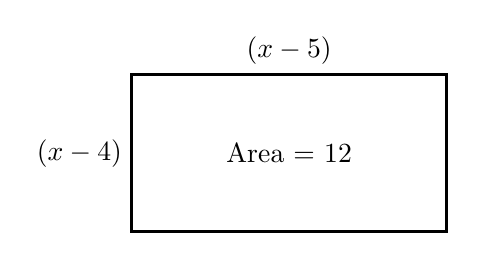
\begin{tikzpicture}
    \draw[very thick] (0,0) rectangle (4,2);
    \node at (2, 0) [below] {};
    \node at (4, 1) [right] {};
    \node at (2, 2) [above] {$(x-5)$};
    \node at (0, 1) [left] {$(x-4)$};
    \node at (2, 1) {Area = 12};
\end{tikzpicture}

\vspace{5cm}
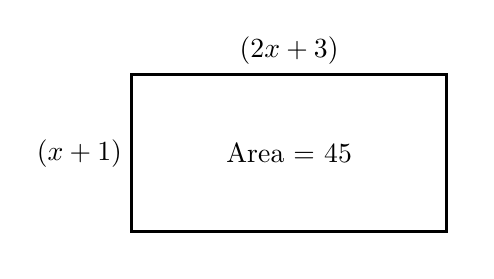
\begin{tikzpicture}
    \draw[very thick] (0,0) rectangle (4,2);
    \node at (2, 0) [below] {};
    \node at (4, 1) [right] {};
    \node at (2, 2) [above] {$(2x+3)$};
    \node at (0, 1) [left] {$(x+1)$};
    \node at (2, 1) {Area = 45};
\end{tikzpicture}

\vspace{5cm}
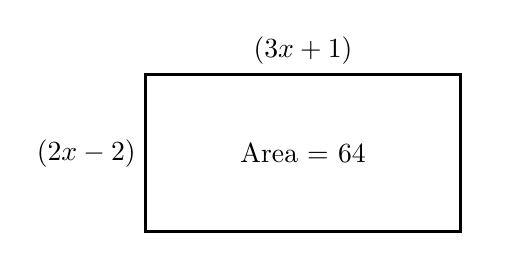
\begin{tikzpicture}
    \draw[very thick] (0,0) rectangle (4,2);
    \node at (2, 0) [below] {};
    \node at (4, 1) [right] {};
    \node at (2, 2) [above] {$(3x+1)$};
    \node at (0, 1) [left] {$(2x-2)$};
    \node at (2, 1) {Area = 64};
\end{tikzpicture}

\end{minipage}

\noindent
Find the vertex for $f(x)=x^2+2x+4$ \\
and it is a min or max?

\end{document}